% \documentclass[table]{beamer}
\documentclass[table,handout]{beamer}
\setbeameroption{show notes}
% \setbeameroption{hide notes}
% \setbeameroption{show only notes}
\usepackage{varwidth}

\newif\ifhide
\newif\ifpost
\newif\ifhideclicker

% \hidetrue
% \hideclickertrue
% \posttrue

\newcommand{\whiteout}[1]{\textcolor{white}{#1}}
% \newcommand{\whiteoutbox}[1]{\fcolorbox{white}{white}{\parbox{\dimexpr \linewidth-2\fboxsep-2\fboxrule}{\whiteout{#1}}}}
% \newcommand{\notebox}[1]{\fcolorbox{blue}{white}{\parbox{\dimexpr \linewidth-2\fboxsep-2\fboxrule}{#1}}}
\newcommand{\whiteoutbox}[1]{\fcolorbox{white}{white}{\parbox{\linewidth}{\whiteout{#1}}}}
\newcommand{\notebox}[1]{\fcolorbox{blue}{white}{\parbox{\linewidth}{#1}}}
\newcommand{\blankbox}[1]{\phantom{\varwidth{\linewidth}\whiteoutbox{#1}\endvarwidth}}
\newcommand{\blank}[1]{\phantom{\varwidth{\linewidth}#1\endvarwidth}}

\ifhide%
    \newcommand{\hmask}[1]{\blank{#1}}%
\else%
    \newcommand{\hmask}[1]{#1}%
\fi

\ifhide%
    \newcommand{\wout}[1]{\whiteout{#1}}%
\else%
    \newcommand{\wout}[1]{#1}%
\fi

\ifhide%
    \newcommand{\hignore}[1]{}%
\else%
    \newcommand{\hignore}[1]{#1}%
\fi

\ifpost%
    \newcommand{\nopost}[1]{}%
\else%
    \newcommand{\nopost}[1]{#1}%
\fi

\ifhideclicker%
    \newcommand{\clickerslide}[1]{\stepcounter{clickerQuestionCounter}%
        \begin{frame}[t]
            \textcolor{blue}{Q \arabic{clickerQuestionCounter}:}
        \end{frame}}
\else%
    \newcommand{\clickerslide}[1]{#1}%
\fi

\ifhide%
    \newcommand{\hidebox}[1]{\blank{#1}}%
\else%
    \newcommand{\hidebox}[1]{\notebox{#1}}%
\fi

\ifhide%
    \newcommand{\wbox}[1]{\whiteoutbox{#1}}%
\else%
    \newcommand{\wbox}[1]{\notebox{#1}}%
\fi

\ifhide%
    \newcommand{\nbox}[1]{\blankbox{#1}}%
\else%
    \newcommand{\nbox}[1]{\notebox{#1}}%
\fi

\ifhideclicker%
    \newcommand{\clickeranswer}[1]{#1}%
\else%
    \ifhide%
        \newcommand{\clickeranswer}[1]{#1}%
    \else%
        \newcommand{\clickeranswer}[1]{\textbf{\textcolor{blue}{#1}}}%
    \fi
\fi

\usepackage{beamerthemesplit}
% \usetheme{boxes}
\usetheme{Malmoe}
\usecolortheme{seahorse}
% \usecolortheme{seagull}
\usepackage{ifthen}
\usepackage{xspace}
\usepackage{multirow}
\usepackage{multicol}
\usepackage{booktabs}
\usepackage{xcolor}
\usepackage{wasysym}
\usepackage{comment}
\usepackage{hyperref}
\hypersetup{pdfborder={0 0 0}, colorlinks=true, urlcolor=blue, linkcolor=blue, citecolor=blue}
\usepackage{changepage}
\usepackage[compatibility=false]{caption}
\captionsetup[figure]{font=scriptsize, labelformat=empty, textformat=simple, justification=centering, skip=2pt}
\usepackage{tikz}
\usetikzlibrary{trees,calc,backgrounds}

\usepackage[bibstyle=joaks-slides,maxcitenames=3,mincitenames=1,backend=biber]{biblatex}

\newrobustcmd*{\shortfullcite}{\AtNextCite{\renewbibmacro{title}{}\renewbibmacro{in:}{}\renewbibmacro{number}{}}\fullcite}

\newrobustcmd*{\footlessfullcite}{\AtNextCite{\renewbibmacro{title}{}\renewbibmacro{in:}{}}\footfullcite}

% Make all footnotes smaller
% \renewcommand{\footnotesize}{\scriptsize}

\definecolor{myGray}{gray}{0.9}
\colorlet{rowred}{red!30!white}

\setbeamertemplate{blocks}[rounded][shadow=true]

\setbeamercolor{defaultcolor}{bg=structure!30!normal text.bg,fg=black}
\setbeamercolor{block body}{bg=structure!30!normal text.bg,fg=black}
\setbeamercolor{block title}{bg=structure!50!normal text.bg,fg=black}

\newenvironment<>{varblock}[2][\textwidth]{%
  \setlength{\textwidth}{#1}
  \begin{actionenv}#3%
    \def\insertblocktitle{#2}%
    \par%
    \usebeamertemplate{block begin}}
  {\par%
    \usebeamertemplate{block end}%
  \end{actionenv}}

\newenvironment{displaybox}[1][\textwidth]
{
    \centerline\bgroup\hfill
    \begin{beamerboxesrounded}[lower=defaultcolor,shadow=true,width=#1]{}
}
{
    \end{beamerboxesrounded}\hfill\egroup
}

\newenvironment{onlinebox}[1][4cm]
{
    \newbox\mybox
    \newdimen\myboxht
    \setbox\mybox\hbox\bgroup%
        \begin{beamerboxesrounded}[lower=defaultcolor,shadow=true,width=#1]{}
    \centering
}
{
    \end{beamerboxesrounded}\egroup
    \myboxht\ht\mybox
    \raisebox{-0.25\myboxht}{\usebox\mybox}\hspace{2pt}
}

\newenvironment{mydescription}{
    \begin{description}
        \setlength{\leftskip}{-1.5cm}}
    {\end{description}}

\newenvironment{myitemize}{
    \begin{itemize}
        \setlength{\leftskip}{-.3cm}}
    {\end{itemize}}

% footnote without a marker
\newcommand\barefootnote[1]{%
  \begingroup
  \renewcommand\thefootnote{}\footnote{#1}%
  \addtocounter{footnote}{-1}%
  \endgroup
}

% define formatting for footer
\newcommand{\myfootline}{%
    {\it
    \insertshorttitle
    \hspace*{\fill} 
    \insertshortauthor, \insertshortinstitute
    % \ifx\insertsubtitle\@empty\else, \insertshortsubtitle\fi
    \hspace*{\fill}
    \insertframenumber/\inserttotalframenumber}}

% set up footer
\setbeamertemplate{footline}{%
    \usebeamerfont{structure}
    \begin{beamercolorbox}[wd=\paperwidth,ht=2.25ex,dp=1ex]{frametitle}%
        % \Tiny\hspace*{4mm}\myfootline\hspace{4mm}
        \tiny\hspace*{4mm}\myfootline\hspace{4mm}
    \end{beamercolorbox}}

% remove navigation bar
\beamertemplatenavigationsymbolsempty

\makeatletter
    \newenvironment{noheadline}{
        \setbeamertemplate{headline}[default]
        \def\beamer@entrycode{\vspace*{-\headheight}}
    }{}
\makeatother

\newcounter{clickerQuestionCounter}
\ifhideclicker%
\newenvironment{clickerquestion}
{ \stepcounter{clickerQuestionCounter}
  \begin{enumerate}[Q \arabic{clickerQuestionCounter}:]\color{white} }
{ \end{enumerate} }
\else%
\newenvironment{clickerquestion}
{ \stepcounter{clickerQuestionCounter}
  \begin{enumerate}[Q \arabic{clickerQuestionCounter}:] }
{ \end{enumerate} }
\fi

\ifhideclicker%
\newenvironment{clickeroptions}
{ \begin{enumerate}[\begingroup\color{white} 1)\endgroup]\color{white} }
{ \end{enumerate} }
\else%
\newenvironment{clickeroptions}
{ \begin{enumerate}[\begingroup\color{red} 1)\endgroup] }
{ \end{enumerate} }
\fi


\tikzstyle{centered} = [align=center, text centered, font=\sffamily\bfseries]
\tikzstyle{skip} = [centered, inner sep=0pt, fill]
\tikzstyle{empty} = [centered, inner sep=0pt]
\tikzstyle{inode} = [centered, circle, minimum width=4pt, fill=black, inner sep=0pt]
\tikzstyle{tnode} = [centered, circle, inner sep=1pt]
\tikzset{
  % edge styles
  level distance=10mm,
  mate/.style={edge from parent/.style={draw,distance=3pt}},
  mleft/.style={grow=left, level distance=10mm, edge from parent path={(\tikzparentnode.west)--(\tikzchildnode.east)}},
  mright/.style={grow=right, level distance=10mm, edge from parent path={(\tikzparentnode.east)--(\tikzchildnode.west)}},
  % node styles
  male/.style={rectangle,minimum size=4mm,fill=gray!80},
  female/.style={circle,minimum size=4mm,fill=gray!80},
  amale/.style={male,fill=red},
  afemale/.style={female,fill=red},
}

\newcommand{\highlight}[1]{\textcolor{violet}{\textit{\textbf{#1}}}}
\newcommand{\super}[1]{\ensuremath{^{\textrm{\sffamily #1}}}}
\newcommand{\sub}[1]{\ensuremath{_{\textrm{\sffamily #1}}}}
\newcommand{\dC}{\ensuremath{^\circ{\textrm{C}}}}
\newcommand{\tb}{\hspace{2em}}
\providecommand{\e}[1]{\ensuremath{\times 10^{#1}}}
\newcommand{\myHangIndent}{\hangindent=5mm}

\newcommand{\spp}[1]{\textit{#1}}

\newcommand\mybullet{\leavevmode%
\usebeamertemplate{itemize item}\hspace{.5em}}

\makeatletter
\newcommand*{\rom}[1]{\expandafter\@slowromancap\romannumeral #1@}
\makeatother

\newcommand{\blankslide}{{\setbeamercolor{background canvas}{bg=black}
\setbeamercolor{whitetext}{fg=white}
\begin{frame}<handout:0>[plain]
\end{frame}}}

\newcommand{\whiteslide}{
\begin{frame}<handout:0>[plain]
\end{frame}}

\newcommand{\f}[1]{\ensuremath{F_{#1}}}
\newcommand{\x}[1]{X\ensuremath{^{#1}}}
\newcommand{\y}[1]{Y\ensuremath{^{#1}}}

% Population growth macros
\newcommand{\popsize}[1]{\ensuremath{N_{#1}}}
\newcommand{\popgrowthratediscrete}[1]{\ensuremath{\lambda_{#1}}}
\newcommand{\popgrowthrate}[1]{\ensuremath{r_{#1}}}
\newcommand{\ptime}{\ensuremath{t}\xspace}

\tikzset{hide on/.code={\only<#1>{\color{white}}}}
\tikzset{
    invisible/.style={opacity=0},
    visible on/.style={alt={#1{}{invisible}}},
    alt/.code args={<#1>#2#3}{%
        \alt<#1>{\pgfkeysalso{#2}}{\pgfkeysalso{#3}}
        % \pgfkeysalso doesn't change the path
    },
}

\bibliography{../bib/references}
\author[J.\ Oaks]{
    %Jamie R.\ Oaks\inst{1}
    Jamie R.\ Oaks
}
\institute[BIOL 180]{
    \inst{}%
        BIOL 180: Introductory Biology
}



\title[Natural Selection]{Evolution by Natural Selection}
% \date{\today}
\date{April 2, 2015}

\begin{document}

\begin{noheadline}
\maketitle
\end{noheadline}

\nopost{
\begin{noheadline}
\begin{frame}[c]
    \vspace{-6mm}
    \begin{center} 
        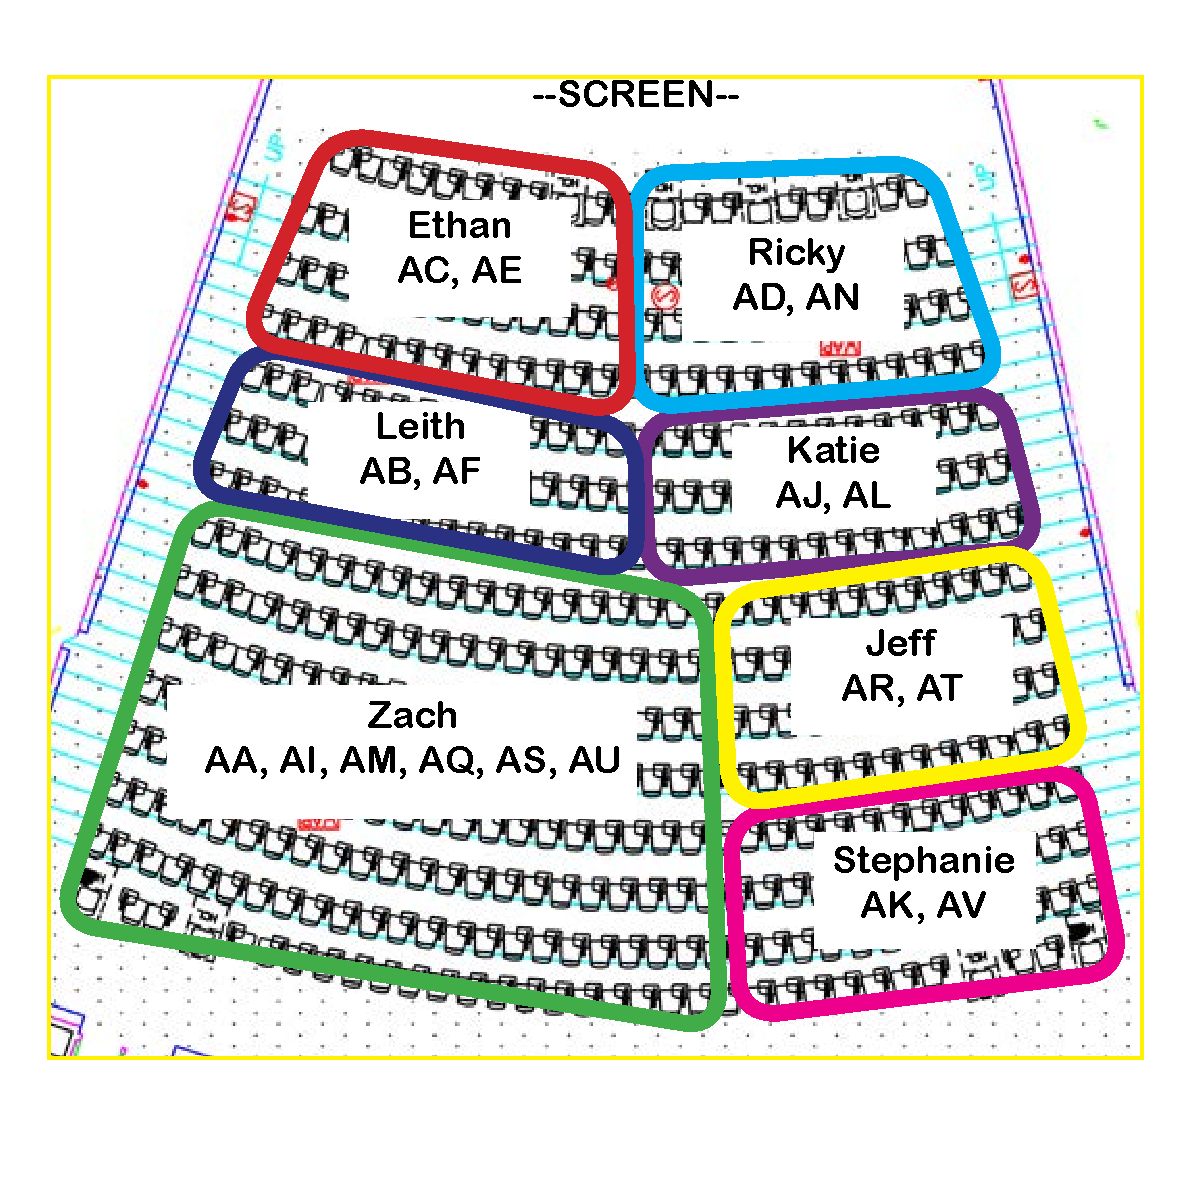
\includegraphics[height=1.3\textheight]{../images/seating-chart.pdf}
    \end{center}
\end{frame}
\end{noheadline}
}

\begin{noheadline}
\begin{frame}
    \begin{clickerquestion}
        \item Which of the following experiments would be the best way to test
            the theory of evolution as formulated by Lamarck?
 
        \begin{clickeroptions}
            \item August Weismann kept mice in identical conditions in the lab
                for 22 generations. Each generation, he cut off their tails.

            \item Follow a population of mice over many generations and record
                (a) any changes that occur in the environment, and (b) any
                corresponding changes in mouse traits. 

            \item \clickeranswer{Keep a population of mice in cold conditions.
                    (In response, the mice will draw their tails up to conserve
                    heat.)  Continue for many generations. Measure tail length
                    each generation.}

            \item Keep a population of mice under identical conditions in the
                lab. Each generation, only allow the mice with the shortest
                tails to breed. 
        \end{clickeroptions}
    \end{clickerquestion}
    \wbox{Weisman actually did this! But, \#3 is more Lamarckian, because
        the mice are making an effort}
\end{frame}
\end{noheadline}

\section{Evolution by Natural Selection}

\begin{noheadline}
\begin{frame}
\frametitle{Today's issues:}
\tableofcontents
\end{frame}
\end{noheadline}

\begin{frame}
    Where do species come from, and how have they come to be so well adapted to
    their environments?

    \begin{quote}
        \ldots a naturalist,
        \uncover<2->{reflecting on the mutual affinities of organic beings,}
        \uncover<3->{on their embryological relations,}
        \uncover<4->{their geographical distribution,}
        \uncover<5->{geological succession,}
        \uncover<6->{and other such facts, might come to the conclusion that
            each species had not been independently created, but had descended
            \ldots from other species.}
        \uncover<7->{Nevertheless, such a conclusion \ldots would be
            unsatisfactory, until it could be shown}
        \uncover<8->{\highlight{HOW} the innumerable species inhabiting this
            world have been modified \ldots}
    \end{quote}
\end{frame}

\begin{frame}[t]
    \frametitle{The pattern}
    \begin{description}
        \item[Evolution:]
            \hmask{The change in the characteristics of a population through time}
    \end{description}
    \note[item]{Pattern: How different from Lamarck? It is NOT progressive}
\end{frame}

\begin{frame}
    \frametitle{The process}

    Darwin’s four postulates explain why/how evolution occurs

    \begin{enumerate}
        \item<2-> Individuals within populations are variable
            \vspace{1cm}

        \item<2-> Some of these variations are passed on to offspring
            \vspace{1cm}

        \item<2-> Not all individuals produce the same number of offspring
            \vspace{1cm}

        \item<2-> Individuals with certain heritable traits produce the most
            offspring
            % \vspace{1cm}
    \end{enumerate}
    \wbox{For each postulate, find example from finches in the textbook, and
        think about how you would test it?}

    \note[item]{Process: How different from Lamarck? It is a process of sorting
        individuals, not transforming individuals}
    \note[item]{\textbf{Emphasize:} individual finches did not change}
\end{frame}

\begin{frame}
    Distill the 4 postulates to their essence
    \vspace{0.5cm}

    Natural selection occurs when:
    \vspace{0.5cm}

    \begin{enumerate}
        \item<2-> Heritable variation
        \vspace{0.5cm}

        \begin{itemize}
            \item<3-> leads to
        \end{itemize}

        \vspace{0.5cm}
        \item<4-> Differential reproductive success 
    \end{enumerate}
    \note[item]{\textbf{Emphasize:} the focus should be on reproduction, not
        survival!}
    % After 2) emphasize that the focus should be on reproduction, not
    % survival; sing It ain’t necessarily so 

    \vspace{0.5cm}
    \uncover<5->{
    \highlight{KEY POINT:} Evolution is simply an outcome (the pattern) of this
    process
    }

\end{frame}

\begin{frame}
    \frametitle{Case history on evolution by natural selection}

    \begin{itemize}
        \item Work in groups of 3; middle person is the scribe
        \item Be sure your names are legible
        \item We're here to answer questions
        \item When you've completed page 1, enter ``1'' on your clicker and
            start the second page
        \item TAs will collect the worksheets
    \end{itemize}
\end{frame}

\begin{frame}
    \begin{enumerate}%[Q 1:]

        \item[Q 2.] Heritable variation in AZT resistance?
        
        \vspace{1cm}
        \item[Q 3.] Differential reproductive success with respect to AZT resistance?

        \vspace{1cm}
        \item[Q 4.] AZT resistance present prior to start of therapy?

        \vspace{1cm}
        \item[Q 5.] Do individual HIV particles change?
    \end{enumerate}
\end{frame}

\begin{frame}
    \frametitle{You need to be able to do this!}

    For any example of change in the characteristics of a population or species
    through time, you should be able to explain how it could happen based on: 

    \begin{enumerate}
        \item<2-> \highlight{Heritable variation} in the trait in question, and 

        \item<3-> \highlight{Differential reproductive success}, based on
            variation in the trait in question (in the context of the
            \highlight{environment}!)
    \end{enumerate}
    \note[item]{Most important concept in 180 (and in biology as a whole)}
\end{frame}

\begin{frame}
    In biology, how do these terms differ from they are used in everyday
    English?
    \begin{description}
        \item[Theory:] \ \\
            \wbox{``speculation'' or something that's ``just an idea'' versus
                ``big'' hypothesis---one that is meant to explain a large chunk
                of the natural world---some theories turn out to be wrong, some
                turn out to be correct}
        \item[Fitness:] \ \\
            \wbox{Being buff versus reproductive success}
            \vspace{1cm}
        \item[Adaptation:] \ \\
            \wbox{Individuals change in response to conditions versus a
                heritable trait that increased fitness in a certain
                environment. Everyday use is Lamarckian---``acclimation''}
    \end{description}
\end{frame}

\section{Darwin's dilemma}

\begin{frame}
    \frametitle{Darwin's dilemma: the problem of variation}

    \uncover<1->{
    The fact of evolution was accepted in the 1870s--1880s.
    }
    
    \bigskip

    \uncover<2->{
    Natural selction an evolutionary process was controversial until 1930s.
    }

    \begin{enumerate}
        \item<3-> Selection will exhaust variation; Why?
            \wbox{\footnotesize Advantageous alleles will go to fixation, then no more
                variation and no more evolution}
            % \vspace{2mm}
        \item<4-> Blending inheritance will eliminate new, advantageous variants; why?
            \wbox{\footnotesize New, rare advantageous variants will blend with the
                common forms of the traits and dilute the advantage---this will
                occur generation after generation until the advantageous trait
                disappears.}
    \end{enumerate}


    \uncover<5->{- Darwin died thinking that his theory was in deep trouble}

    \uncover<6->{- Solution had been published years before in 1865---Next
        class!}
\end{frame}

\end{document}

